\chapter{Introducción específica} % Main chapter title

\label{Chapter2}

%----------------------------------------------------------------------------------------
%	SECTION 1
%----------------------------------------------------------------------------------------
En este capítulo se presenta una introducción técnica a la temática abordada en el trabajo. 

\section{Requerimientos}
\label{sec:ejemplo}
A continuación, se detallan los principales requerimientos funcionales y técnicos.

\subsection*{Requerimientos funcionales}

\begin{itemize}
\item Obtener series temporales de cobertura de agua superficial en el Salar de Llullaillaco, a partir de índices espectrales derivados de imágenes Landsat.
\item Correlacionar los patrones de presencia de agua con variables climáticas globales asociadas al ENSO (Niño 3.4, SOI, MEI).
\item Generar modelos predictivos de ocurrencia de agua mediante el uso algoritmos de aprendizaje supervisado.
\item Visualizar los resultados mediante mapas y gráficos temporales que permitan interpretar los patrones hidrológicos en relación con el clima.
\end{itemize}

\subsection*{Requerimientos técnicos}

\begin{itemize}
\item Acceso a la plataforma Google Earth Engine (GEE) para el procesamiento de imágenes satelitales Landsat 5, 7 y 8.
\item Dataset mensual de los índices climáticos de ENSO: Niño 3.4, \textit{Southern Oscillation Index (SOI)}, y \textit{Multivariate ENSO Index (MEI)}.
\item Computadora con entorno de desarrollo Python, con acceso a bibliotecas como \texttt{PANDAS, NUMPY, MATPLOTLIB, SKLEARN, TORCH}.
\item Conexión a Internet para descarga de datos y acceso a \textit{notebooks} en la nube.
\end{itemize}



%----------------------------------------------------------------------------------------
%	SECTION 2
%----------------------------------------------------------------------------------------

\section{Técnicas utilizadas}

El desarrollo de este trabajo se basa en la combinación de técnicas de teledetección, análisis multitemporal y aprendizaje automático, integradas en un flujo de trabajo que permite monitorear la presencia de agua superficial en el Salar de Llullaillaco y explorar su relación con la variabilidad climática regional.

\subsection{Google Earth Engine (GEE)}

Se utilizó la plataforma GEE para el acceso y procesamiento de imágenes Landsat 5, 7 y 8, con el mismo enfoque usado por \cite{ferran2024ceia, roldan2023ceia}. GEE permite aplicar filtros temporales, máscaras de nubes, recortes espaciales y cálculos de índices espectrales sobre áreas definidas, con eficiencia y escalabilidad.


\subsection{Sobre los índices espectrales}

El índice espectral utilizado en este trabajo fue el NDWI (\textit{Normalized Difference Water Index}). Este índice se basa en relaciones matemáticas entre bandas del espectro electromagnético que capturan variaciones en la reflectancia del terreno. Estas métricas se fundamentan en estudios de respuesta espectral diferencial de distintos tipos de cobertura superficial, como agua, vegetación o nieve, especialmente visibles en las bandas verde, roja, infrarroja cercana (NIR) y de onda corta (SWIR).

Tal como se observa en trabajos clásicos de teledetección \cite{tucker1979red, huete1988soil}, la vegetación sana refleja fuertemente en el infrarrojo cercano y absorbe en la banda roja, mientras que el agua y la nieve presentan perfiles espectrales contrastantes. Estas propiedades permiten construir índices que destacan las coberturas de interés.


En este trabajo se usó principalmente NDWI como un marco conceptual útil para entender las diferencias espectrales de las cubiertas superficiales analizadas en el Salar de Llullaillaco.


\subsection{Índice espectral utilizado}

El indice NDWI permite caracterizar el comportamiento espectral del suelo y del agua en ambientes de alta reflectancia como los salares. El NDWI resalta la presencia de agua superficial ya que emplea las bandas del verde y el infrarrojo cercano (NIR). Su expresión matemática se observa en la ecuación \ref{eq:ndwi}.

    \begin{equation}
        \label{eq:ndwi}
        NDWI = \frac{\text{Green} - \text{NIR}}{\text{Green} + \text{NIR}}
    \end{equation}

% \begin{figure}[htpb]
% 	\centering
% 	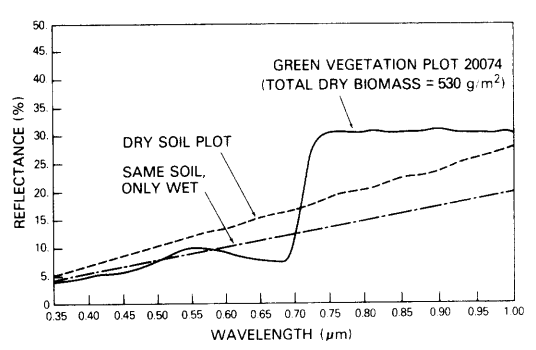
\includegraphics[scale=.5]{Figures/fig3.png}
% 	\caption{Reflectancias espectrales de suelo seco, suelo húmedo y vegetación completamente verde\protect\footnotemark.}
% 	\label{fig:curva_ref}
% \end{figure}  
% \newpage
% \footnotetext{Imagen tomada de \cite{tucker1979red}.}}


\subsection{Imágenes Landsat utilizadas}

Para este trabajo se emplearon imágenes ópticas de las misiones \Landsat 5 TM y Landsat 8 OLI, disponibles en la plataforma GEE como colecciones. Las colecciones empleadas de Google Earth Engine fueron:

% \begin{itemize}
%     \item \texttt{LANDSAT/LT05/C02/T1\_L2} — Landsat 5 TM, colección nivel 2 (surface reflectance).
%     \item \texttt{LANDSAT/LE07/C02/T1\_L2} — Landsat 7 ETM+, colección nivel 2.
%     \item \texttt{LANDSAT/LC08/C02/T1\_L2} — Landsat 8 OLI, colección nivel 2.
% \end{itemize}

Estas imágenes corresponden a productos de nivel 2, que incluyen correcciones atmosféricas (Surface Reflectance) y enmascaramiento de nubes mediante algoritmos QA/QC. Se seleccionaron todas las escenas disponibles y se priorizaron aquellas sin nubes y con cobertura adecuada del Salar de Llullaillaco.

Las bandas empleadas en los cálculos de índices espectrales fueron:

\begin{table}[H]
\centering
\caption{Bandas utilizadas en las misiones Landsat seleccionadas.}
\label{tab:landsat_bandas}
\begin{tabular}{lcccc}
\toprule
Misión & Green & Red & NIR & SWIR1 \\
\midrule
Landsat 5 TM  & Banda 2 & Banda 3 & Banda 4 & Banda 5 \\
Landsat 8 OLI & Banda 3 & Banda 4 & Banda 5 & Banda 6 \\
\bottomrule
\end{tabular}
\end{table}



Estas bandas fueron utilizadas para calcular el índice NDWI. Se ajustaron sus combinaciones según el sensor. La consistencia intersensorial fue manejada a través de normalización espectral mensual y máscaras de calidad provistas por GEE.


\subsection{U-Net y su aplicación en la clasificación de cuerpos de agua}

La \textit{U-Net} es una arquitectura de redes neuronales convolucionales diseñada para
segmentación semántica de imágenes. Su estructura en forma de ``U'' combina un
proceso de codificación, que extrae características de alto nivel reduciendo la
resolución espacial, con un proceso de decodificación que reconstruye la
segmentación a la resolución original. Los \textit{skip connections} permiten
recuperar detalles finos en los bordes, logrando una clasificación más precisa.

En el caso de cuerpos de agua, la U-Net presenta ventajas frente a métodos
puramente espectrales como el NDWI. Permite diferenciar con mayor exactitud
zonas de agua en ambientes heterogéneos, reduciendo falsos positivos asociados
a sombras o suelos húmedos. Trabajos recientes, como \textit{DeepAqua}\cite{DeepAqua2023},
utilizan el NDWI como \textit{teacher} para generar etiquetas binarias y entrenar
una U-Net como \textit{student}, demostrando que incluso con etiquetas automáticas
se obtiene una segmentación robusta y generalizable en imágenes Landsat y Sentinel.


\subsection{Conocimiento distilado para segmentación de agua}

El esquema de \textit{knowledge distillation} (KD) aplicado a cartografía de agua consiste en entrenar un \textit{student} de segmentación profunda a partir de etiquetas proxy generadas automáticamente por un \textit{teacher}. 

En la línea de \emph{DeepAqua} \cite{DeepAqua2023}, el \textit{teacher} se construye en el dominio óptico mediante el índice NDWI y el \textit{student} es una red neuronal profunda de tipo U-Net que aprende a reproducir dichas máscaras, evitando anotación manual.

El NDWI \textit{teacher} y se umbraliza para obtener una máscara binaria. Opcionalmente se aplican operaciones morfológicas ligeras para eliminar ruido. 

En este trabajo el teacher se genera con imágenes Landsat con control de nubosidad y sincronización temporal mensual como se explicó anteriormente.

Para sección \textit{Student} (U-Net) empleamos una U-Net 2D estándar con \emph{skip connections}. La entrada es una imagen multicanal y la salida es una binaria de agua/no-agua. 

En el trabajo \cite{DeepAqua2023} la entrada es SAR (C-band) y el modelo aprende a partir del teacher óptico (máscara binaria a partir de NDWI). En nuestra adaptación usamos bandas ópticas Landsat (SR5--SR4--SR3) como entrada, manteniendo la misma función objetivo y protocolo de entrenamiento. Esta variante conserva las ventajas de KD (eliminar rotulado manual) y simplifica la disponibilidad operativa de imágenes SAR.

% --- Figura (opcional) ---
\begin{figure}[t]
  \centering
  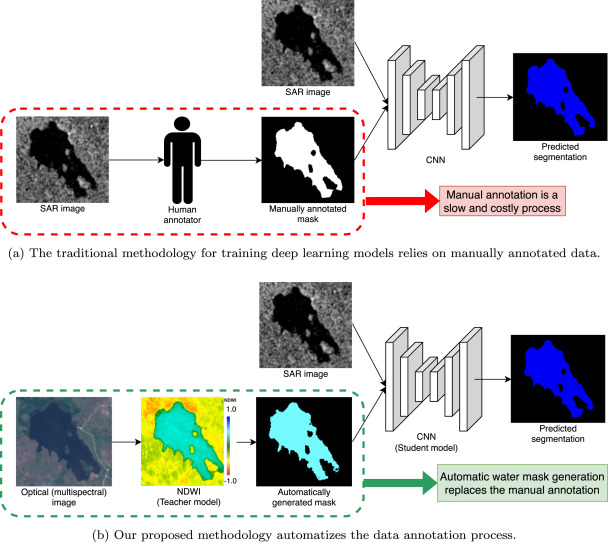
\includegraphics[scale=0.7]{Figures/KD_deepaqua.jpg}
  \caption{Esquema de distillation para segmentación de agua. Arriba: enfoque tradicional con anotación manual. Abajo: enfoque teacher - student con U-Net. \protect\footnotemark.}
  \label{fig:kd-water}
\end{figure}
\FloatBarrier 

\footnotetext{Imagen tomada de \cite{DeepAqua2023}.}

De esta manera el KD reduce la dependencia de rótulos manuales, mejora la robustez ante variabilidad espectral y permite operación \emph{near real-time}. En \cite{DeepAqua2023} se reportan mejoras en IoU/F1 frente a métodos puramente no supervisados y capacidad para capturar agua abierta y vegetada; en nuestra adaptación óptica, el comportamiento esperado es comparable en escenas despejadas, con el costo de una mayor sensibilidad a nubosidad (mitigado vía filtrado y composición mensual).



\subsection*{Variables climáticas ENSO}

El fenómeno El Niño-Oscilación del Sur (ENSO) es uno de los principales moduladores del clima a escala interanual y tiene un impacto significativo en los regímenes de precipitación y temperatura en América del Sur. ENSO es un sistema acoplado océano-atmósfera que alterna entre tres fases:

\begin{itemize}
    \item El Niño: fase cálida, asociada a un aumento de la temperatura superficial del mar (SST) en el Pacífico ecuatorial central y oriental.
    \item La Niña: fase fría, caracterizada por anomalías negativas de SST en la misma región.
    \item Neutral: ausencia de anomalías significativas en las condiciones oceánicas y atmosféricas.
\end{itemize}

Estas variaciones alteran la circulación atmosférica a nivel planetario, incluyendo la intensidad de los vientos alisios, el transporte de humedad y la posición de la Zona de Convergencia Intertropical (ZCIT). En regiones como la Puna argentina, se ha documentado que las fases de ENSO afectan directamente los patrones de precipitación y, por ende, la disponibilidad de agua superficial y la recarga de los salares.

Para capturar cuantitativamente la influencia de ENSO, en este trabajo se utilizaron tres índices climáticos de carácter mensual:

\begin{itemize}
    \item Niño 3.4 Index (ONI): representa la anomalía mensual de la SST en la región 5° N – 5° S, 170° W – 120° W. Es el indicador principal utilizado por la NOAA para clasificar eventos ENSO. Se calcula como una media móvil de tres meses de anomalías de SST basadas en el conjunto de datos ERSST.v5. Valores $\geq 0{,}5\,^{\circ}\text{C}$ mantenidos durante al menos cinco trimestres móviles consecutivos definen un evento El Niño, mientras que valores $\geq 0{,}5\,^{\circ}\text{C}$ definen un evento La Niña \parencite{noaaONI}.
    
    \item Southern Oscillation Index (SOI): se calcula a partir de la diferencia estandarizada de presión atmosférica entre Tahití y Darwin, Australia. Valores positivos (por encima de +7) se asocian a La Niña, valores negativos (por debajo de -7) a El Niño, mientras que valores intermedios se consideran neutrales. Este índice es publicado por el \textit{Australian Bureau of Meteorology} \parencite{bom_soi_2024}.
    
    \item Multivariate ENSO Index (MEI.v2): combina seis variables atmosféricas y oceánicas (SST, presión al nivel del mar, vientos zonales y meridionales, temperatura del aire y nebulosidad baja) mediante análisis de componentes principales. Esto permite capturar interacciones complejas del sistema acoplado océano-atmósfera. El MEI se calcula de manera bimestral móvil y se considera que valores superiores a +0,5 indican El Niño, inferiores a -0,5 indican La Niña y valores intermedios corresponden a condiciones neutras \parencite{meiindex}.
\end{itemize}

Estos indicadores, obtenidos de fuentes oficiales como la \textit{NOAA Climate Prediction Center}, el \textit{Physical Sciences Laboratory} de EE.UU. y el \textit{Bureau of Meteorology} de Australia, se utilizaron como variables explicativas en este estudio. Su inclusión permite explorar cómo las oscilaciones oceánicas y atmosféricas globales se reflejan en la variabilidad de agua superficial en el Salar de Llullaillaco, aportando un marco climático regional al análisis hidrológico local.


%----------------------------------------------------------------------------------------
%	SECTION 3
%----------------------------------------------------------------------------------------

\section{Herramientas y bibliotecas utilizadas}

En el flujo de trabajo se emplearon diversas bibliotecas de Python y plataformas en la nube. 
A continuación se listan las principales:

\begin{itemize}
    \item \texttt{Python 3.10}, \texttt{pandas}, \texttt{numpy}, \texttt{matplotlib}, \texttt{seaborn}, \texttt{scikit-learn}, \texttt{pytorch}: bibliotecas estándar de análisis de datos, visualización y aprendizaje automático.
    \item \texttt{xarray}: manejo de cubos n–dimensionales (\textit{Dataset}/\textit{DataArray}), resampleo temporal y álgebra raster \parencite{xarray2020}.
    \item \texttt{rioxarray}: gestión de CRS, reproyección, recorte espacial y cálculo en unidades métricas (e.g., EPSG:22173) \parencite{rioxarray}.
    \item \texttt{xee}: integración directa GEE~$\leftrightarrow$~xarray preservando \texttt{crs} y \texttt{scale}.
    \item \texttt{geemap}: visualización interactiva de colecciones GEE en notebooks, dibujo de ROI y exportación/inspección de capas \parencite{geemap2021}.
    \item \texttt{Google Earth Engine API (Python)}: cliente oficial para consultas y procesamiento remoto de colecciones satelitales \parencite{gorelick2017gee}.
    \item \texttt{Google Colab}: entorno de ejecución en la nube empleado para la integración con GEE y el entrenamiento de modelos.
\end{itemize}

Además, se utilizaron funciones propias escritas en Python para carga de datos, limpieza, ingeniería de variables y evaluación de modelos.




%----------------------------------------------------------------------------------------